\documentclass[11pt,a4paper]{article}

\usepackage[T1]{fontenc}
\usepackage[utf8]{inputenc}
\usepackage[italian]{babel}
\usepackage{lmodern}
\usepackage[a4paper,margin=2.5cm]{geometry}
\usepackage{amsmath,amssymb}
\usepackage{graphicx}
\usepackage{booktabs}
\usepackage{array}
\usepackage{caption}
\usepackage{enumitem}
\usepackage{tikz}
\usetikzlibrary{arrows.meta,positioning}
\usepackage[hidelinks]{hyperref}

\newcommand{\Emin}{E_{\min}}
\newcommand{\zconf}{z_{\text{conf}}}
\newcommand{\zseq}{z_{\text{seq}}}

\title{Decoy discriminator per il modello HP 2D}
\author{Alessandro Bado}
\date{\today}

\begin{document}

\maketitle

% \begin{abstract}
% Riassunto di poche righe: problema, metodo, risultato principale.
% \end{abstract}

% =====================================================================
\section{Introduzione}
\label{sec:intro}

\subsection{Contesto}
\label{sec:contesto}

Una proteina è una catena lineare di amminoacidi che, in ambiente fisiologico, si ripiega spontaneamente in una struttura tridimensionale specifica, detta \textbf{stato nativo}. Dalla struttura nativa dipende la funzione della proteina.

Secondo l'ipotesi termodinamica di Anfinsen~\cite{anfinsen1973}, la struttura nativa è determinata dalla sola sequenza e corrisponde al minimo globale dell'energia libera. Prevedere il folding equivale quindi a cercare la conformazione di energia minima tra un numero di alternative che cresce in modo esponenziale con la lunghezza della catena.

Con modelli atomistici questa ricerca è molto costosa. Per studiare i principi generali del folding si usano allora \textbf{modelli semplificati su reticolo}, che riducono la proteina all'essenziale e rendono il problema trattabile al calcolatore.

\subsection{Il modello HP}
\label{sec:hp}

Il modello \textbf{HP} (idrofobico-polare), proposto da Dill nel 1985~\cite{dill1985}, è il più noto tra i modelli su reticolo. Si basa sull'osservazione che la forza principale del folding è l'effetto idrofobico. In questo contesto, i residui apolari tendono a raccogliersi all'interno della proteina, lontano dal solvente.

Nel modello ogni amminoacido è ridotto a uno di due tipi, \textbf{H} (idrofobico) o \textbf{P} (polare), e la proteina diventa una stringa come \texttt{PHHPPHPPHHPPHHPP}. Una conformazione è un cammino autoevitante sul reticolo quadrato 2D in cui residui consecutivi occupano nodi adiacenti e nessun nodo è occupato due volte.

L'energia della configurazione proteica viene calcolata contando i contatti H--H, cioè le coppie di residui H adiacenti sul reticolo ma non consecutivi nella catena:
\begin{equation}
  E(c) = -\sum_{i < j - 1} \delta_{H}(i)\, \delta_{H}(j)\, \Delta(r_i, r_j)
  \label{eq:energia}
\end{equation}
dove $\delta_H(i)$ vale 1 se il residuo $i$ è di tipo H, e $\Delta(r_i, r_j)$ vale 1 se le posizioni $r_i$ e $r_j$ sono adiacenti sul reticolo. Lo stato nativo è la conformazione con l'energia più bassa la quale, spesso, non è unica, perché più conformazioni degeneri possono raggiungere lo stesso minimo.

Nonostante la semplicità, trovare il minimo nel modello HP è un problema NP-difficile. Per questo si usano metodi stocastici come il \textbf{Replica Exchange Monte Carlo} (REMC), che in questo progetto segue la variante di Thachuk et al.\ (2007)~\cite{thachuk2007}.

\subsection{Obiettivi}
\label{sec:obiettivi}

L'obiettivo del progetto è capire se un algoritmo stocastico di ricerca del minimo che esplora il paesaggio energetico di una sequenza (nel nostro caso il REMC) sia in grado di produrre un dataset valido per addestrare un modello di machine learning. Il modello, data in ingresso una sequenza HP e una sua conformazione, deve stabilire se la conformazione è \textbf{nativa} oppure un \textbf{decoy}.

Un decoy è una conformazione plausibile della sequenza che però non corrisponde allo stato nativo. Durante la ricerca il REMC visita sia le conformazioni di energia minima, che diventano gli esempi nativi, sia molte conformazioni a energia più alta, da cui si estraggono i decoy.

Il compito non è banale perché l'energia da sola non basta siccome lo stesso valore di $E(c)$ può essere il minimo per una sequenza e lontano dal minimo per un'altra. Il modello riceve solo la sequenza e le coordinate della conformazione, non l'energia minima, quindi deve ricavare due informazioni:
\begin{itemize}
  \item \textbf{dalla sequenza}, quanto in basso può arrivare l'energia, in base al numero e alla posizione dei residui H lungo la catena (l'energia minima);
  \item \textbf{dalla forma della conformazione}, se questa ha le caratteristiche di uno stato nativo.
\end{itemize}

Una volta addestrato, il modello risponde con un solo passaggio della rete, senza rieseguire il REMC su ogni nuova sequenza.

Il lavoro si articola in tre passi:
\begin{enumerate}
  \item \textbf{Generazione del dataset} con il REMC, con l'energia minima verificata per enumerazione esatta (sezioni~\ref{sec:remc} e~\ref{sec:dataset}).
  \item \textbf{Modello di classificazione}, che combina una rete neurale su grafo (GNN) applicata ai contatti della conformazione con una rete convoluzionale 1D (CNN) applicata alla sequenza (sezione~\ref{sec:modello}).
  \item \textbf{Valutazione.} Il dataset è considerato valido se il modello generalizza a sequenze mai viste in addestramento. Le prestazioni sono confrontate con tre baseline più semplici (sezioni~\ref{sec:training} e~\ref{sec:risultati}).
\end{enumerate}

% =====================================================================

\section{Algoritmo REMC}
\label{sec:remc}

\subsection{Perché non basta un Monte Carlo semplice}
\label{sec:mc}

Il REMC estende il \textbf{Monte Carlo Metropolis}, che esplora le conformazioni proteiche con piccole mosse locali. Una mossa che porta l'energia da $E$ a $E'$, con $\Delta E = E' - E$, viene accettata con probabilità:
\begin{equation}
  P_{acc} =
  \begin{cases}
    1 & \text{se } \Delta E \le 0 \\
    e^{-\Delta E / T} & \text{se } \Delta E > 0
  \end{cases}
  \label{eq:metropolis}
\end{equation}
dove $T$ è la temperatura (con $k_B = 1$).

Il paesaggio energetico del modello HP è però \textbf{rugoso}, con molti minimi locali separati da barriere. Il risultato dipende quindi molto dalla temperatura:
\begin{itemize}
  \item \textbf{a $T$ bassa} la catena si compatta in fretta, ma resta intrappolata nel primo minimo locale che incontra, per esempio una struttura compatta con il nucleo H nella posizione sbagliata;
  \item \textbf{a $T$ alta} la catena supera le barriere, ma accetta troppe mosse sfavorevoli e non si assesta sul minimo.
\end{itemize}

Nessuna temperatura singola concilia le due esigenze. Il REMC risolve il problema facendo lavorare insieme più simulazioni a temperature diverse.

\subsection{Repliche e scambi}
\label{sec:repliche}

Il REMC simula $M$ copie della stessa sequenza, dette \textbf{repliche}, ognuna a una temperatura fissa. Le temperature sono equispaziate tra $T_1$ (la più fredda) e $T_M$ (la più calda):
\begin{equation}
  T_k = T_1 + (k - 1)\,\frac{T_M - T_1}{M - 1}, \qquad k = 1, \dots, M
  \label{eq:temperature}
\end{equation}

La simulazione procede per \textbf{cicli}. In ogni ciclo:
\begin{enumerate}
  \item ogni replica esegue $\varphi$ passi Metropolis alla propria temperatura, secondo l'equazione~\eqref{eq:metropolis};
  \item si propongono scambi di conformazione tra repliche a temperature adiacenti.
\end{enumerate}

Ogni passo Metropolis propone una mossa locale su un residuo scelto a caso con probabilità $\rho$ per una \textbf{pull move}~\cite{lesh2003}, la quale resta possibile anche nelle conformazioni compatte, altrimenti una mossa \textbf{VSHD} (end, corner o crankshaft).

Lo scambio tra le repliche $i$ e $j$, con energie $E_i$, $E_j$ e temperature inverse $\beta = 1/T$, viene accettato con probabilità:
\begin{equation}
  P_{swap} = \min\left(1,\; e^{(\beta_i - \beta_j)(E_i - E_j)}\right)
  \label{eq:swap}
\end{equation}

In questo modo una conformazione trovata da una replica calda può scendere fino alla replica fredda, che la rifinisce verso il minimo. Al contrario, una conformazione intrappolata a bassa temperatura può salire, ``sciogliersi'' e uscire dal minimo locale.

\subsection{Parametri}
\label{sec:parametri}

Per generare il dataset, il REMC viene eseguito una volta per ciascuna delle 2000 sequenze, partendo dalla catena distesa su un reticolo $20 \times 20$. Nella tabella~\ref{tab:parametri} sono riportati i parametri di ingresso dell'algoritmo.

\begin{table}[htbp]
  \centering
  \caption{Parametri del REMC usati per generare il dataset.}
  \label{tab:parametri}
  \begin{tabular}{lcc}
    \toprule
    Parametro & Simbolo & Dataset del progetto \\
    \midrule
    Numero di repliche     & $M$       & 5     \\
    Temperatura minima     & $T_1$     & 0,160 \\
    Temperatura massima    & $T_M$     & 0,600 \\
    Passi locali per ciclo & $\varphi$ & 100   \\
    Numero di cicli        & ---       & 500   \\
    \bottomrule
  \end{tabular}
\end{table}

Un seme diverso per ogni sequenza rende ogni esecuzione indipendente e riproducibile.

\subsection{Verifica esatta}
\label{sec:verifica}

Il REMC è un metodo stocastico e non garantisce di trovare il minimo globale. Per le sequenze fino a 20 residui, quindi per tutte quelle del dataset, $\Emin$ viene confrontata con il minimo vero calcolato per \textbf{enumerazione esatta} di tutte le conformazioni. Una sequenza viene scartata in due casi:
\begin{itemize}
  \item il REMC non ha raggiunto il minimo vero ovvero i suoi ``nativi'' sarebbero in realtà decoy;
  \item $\Emin = 0$, cioè nessuna conformazione forma contatti H--H e tutte sarebbero native.
\end{itemize}

Così l'energia di ogni esempio etichettato come nativo è certamente quella minima.

\section{Generazione del dataset}
\label{sec:dataset}

Il dataset è formato da coppie (sequenza, conformazione) con un'etichetta binaria:
\begin{itemize}
  \item \textbf{1} se la conformazione è nativa;
  \item \textbf{0} se è un decoy.
\end{itemize}
Tutte le conformazioni provengono dalle esecuzioni del REMC descritte nella sezione~\ref{sec:remc}.

Le sequenze sono 2000, di 16 residui, generate a caso in cui ogni residuo è H con probabilità 0,5. Una sequenza e la sua inversa descrivono la stessa catena letta dall'altro capo, quindi se ne tiene una sola delle due. Le sequenze scartate dalla verifica della sezione~\ref{sec:verifica} vengono sostituite da nuove sequenze, finché non se ne ottengono 2000 valide.

Per ogni sequenza si raccolgono:
\begin{itemize}
  \item le \textbf{traiettorie}, cioè ogni conformazione accettata durante la simulazione;
  \item le \textbf{istantanee} di tutte le repliche (per ogni temperatura), salvate ogni 2 cicli.
\end{itemize}

Due conformazioni che differiscono solo per una traslazione, una rotazione o una riflessione del reticolo hanno la stessa energia e la stessa forma. Per questo ogni conformazione è ridotta a una \textbf{forma canonica} e gli stati equivalenti contano una volta sola.

\subsection{Conformazioni native}
\label{sec:nativi}

Sono native tutte le conformazioni distinte che il REMC ha visitato all'energia minima $\Emin$ della sequenza. Il dataset contiene quindi tutti gli stati \textbf{degeneri} trovati, non solo la migliore conformazione restituita dall'algoritmo. Per non sbilanciare il dataset verso le sequenze molto degeneri, si tengono al massimo \textbf{20 nativi per sequenza}, scelti a caso quando il REMC ne ha trovati di più.

Grazie alla verifica della sezione~\ref{sec:verifica}, ogni nativo è davvero uno stato di energia minima e ogni decoy ha energia strettamente maggiore di $\Emin$.

\subsection{Decoy e fasce di difficoltà}
\label{sec:fasce}

Per ogni decoy, si calcola il \textbf{gap} dal minimo:
\begin{equation}
  g(c) = E(c) - \Emin
  \label{eq:gap}
\end{equation}

Un decoy con gap piccolo è quasi nativo ed è difficile da distinguere, mentre uno con gap grande è lontano dal minimo ed è facile. Lo stesso gap però pesa in modo diverso a seconda della sequenza infatti un gap di 2 è grande se $\Emin = -3$ mentre è piccolo se $\Emin = -9$. Per questo le fasce (tabella~\ref{tab:fasce}) si basano sul gap \textbf{relativo} $g / |\Emin|$, che vale 0 per un nativo e 1 per una conformazione senza contatti H--H.

\begin{table}[htbp]
  \centering
  \caption{Fasce di difficoltà dei decoy.}
  \label{tab:fasce}
  \begin{tabular}{lll}
    \toprule
    Fascia & Gap relativo $g / |\Emin|$ & Difficoltà \\
    \midrule
    near & fino a 0,34 (oppure $g = 1$) & alta  \\
    mid  & da 0,34 a 0,67               & media \\
    far  & oltre 0,67                   & bassa \\
    \bottomrule
  \end{tabular}
\end{table}

Ogni sequenza riceve tanti decoy quanti sono i suoi nativi, divisi in parti uguali tra le tre fasce. Se una fascia non ha abbastanza candidati, i decoy mancanti vengono presi dalle altre. Dentro ogni fascia i decoy sono scelti a caso.

\subsection{Trappole cinetiche}
\label{sec:trappole}

Una \textbf{trappola cinetica} è un minimo locale dell'energia rispetto all'insieme delle mosse in cui nessuna singola mossa, VSHD o pull move, abbassa l'energia della conformazione. Indicato con $N(c)$ l'insieme delle conformazioni raggiungibili da $c$ con una mossa, $c$ è una trappola se:
\begin{equation}
  E(c') \ge E(c) \quad \forall\, c' \in N(c)
  \label{eq:trappola}
\end{equation}

Sono gli stati in cui un Monte Carlo a bassa temperatura resta bloccato. Di solito sono conformazioni compatte, con molti contatti H--H ma con il nucleo idrofobico nella posizione sbagliata. Per il modello sono i decoy più difficili, perché somigliano a uno stato nativo.

Per questo metà della quota della fascia near è riservata alle trappole, cercate tra i primi 200 candidati near di ogni sequenza. Se non ce ne sono abbastanza, la quota viene completata con altri decoy near. Ogni decoy porta un indicatore che dice se è una trappola, così nei risultati si può misurare a parte quanto il modello sbaglia su questi casi.

\subsection{Bilanciamento e suddivisione}
\label{sec:split}

Il bilanciamento è \textbf{1:1 per sequenza}, non solo sul totale. Se una sequenza avesse più nativi che decoy, il modello potrebbe imparare che quella sequenza è ``spesso nativa'' invece di guardare la conformazione.

La suddivisione in train, validation e test (80\%, 10\%, 10\%) è fatta \textbf{per sequenza}, ovvero tutte le conformazioni di una sequenza finiscono nello stesso insieme. Il test contiene quindi 200 sequenze mai viste in addestramento, e misura proprio la capacità di generalizzare richiesta dagli obiettivi. Una suddivisione per conformazione metterebbe invece nativi della stessa sequenza sia in train sia in test, e il modello potrebbe riconoscerli a memoria.

\section{Modello di classificazione}
\label{sec:modello}

Il classificatore riceve una sequenza HP e una sua conformazione e restituisce la probabilità che la conformazione sia nativa, cioè che $E(c) = \Emin$. Come visto nella sezione~\ref{sec:obiettivi}, il problema si scompone in due parti: 
\begin{enumerate}
    \item Stimare l'energia $\boldsymbol{E(c)}$, proprietà \emph{locale} che dipende solo dai contatti H--H della conformazione
    \item Stimare l'energia minima $\boldsymbol{\Emin}$, proprietà \emph{globale} che dipende solo dalla stringa HP.
\end{enumerate}

Il modello riflette questa scomposizione con due rami separati, uno per la conformazione e uno per la sequenza, i cui risultati vengono combinati da un classificatore finale.

\subsection{Rappresentazione dell'input}
\label{sec:input}

\paragraph{Sequenza.} La sequenza di $N = 16$ residui è codificata come vettore binario $h$, con $h_i = 1$ se il residuo $i$ è di tipo H. A ogni residuo sono associate quattro caratteristiche calcolate dalla sola sequenza:
\begin{itemize}
  \item il tipo (H o P);
  \item la \textbf{parità} dell'indice $i$;
  \item la posizione lungo la catena, normalizzata come $i / (N - 1)$;
  \item un indicatore che vale 1 per i due estremi della catena.
\end{itemize}

\paragraph{Conformazione.} Le coordinate dei residui sul reticolo non sono usate direttamente ma vengono convertite nella \textbf{mappa dei contatti} $C$, una matrice $N \times N$ con $C_{ij} = 1$ se i residui $i$ e $j$ sono adiacenti sul reticolo ma non consecutivi nella catena. Questa rappresentazione è invariante per traslazioni, rotazioni e riflessioni della conformazione, che non ne cambiano l'energia.

La conformazione diventa così un \textbf{grafo} in cui i nodi sono i residui e gli archi sono di due tipi:
\begin{itemize}
  \item i \textbf{legami} tra residui consecutivi $(i, i + 1)$, uguali per tutte le conformazioni;
  \item i \textbf{contatti} topologici dati da $C$, che distinguono una conformazione dall'altra.
\end{itemize}

\subsection{Architettura GNN + CNN 1D}
\label{sec:architettura}

Il modello principale ha due rami, uno per ciascun sotto-problema, e tre teste di uscita.

\paragraph{Ramo della conformazione (GNN).} Una rete neurale su grafo (Graph Neural Network) elabora il grafo della conformazione. Ogni residuo $i$ è descritto da un vettore $h_i$ di dimensione 64, inizializzato con una trasformazione lineare delle sue caratteristiche. In ciascuno dei 4 strati di \emph{message passing} ogni residuo riceve un messaggio da ogni vicino, con pesi diversi per legami e contatti:
\begin{equation*}
  m_i = \sum_{j} B_{ij} \, W_b \, h_j + \sum_{j} C_{ij} \, W_c \, h_j
\end{equation*}
dove $B$ è la matrice dei legami e $C$ la mappa dei contatti. Il vettore del residuo viene poi aggiornato combinando il suo valore con la somma dei messaggi:
\begin{equation*}
  h_i \leftarrow \mathrm{LayerNorm}\left(h_i + \mathrm{MLP}\left([\,h_i,\; m_i\,]\right)\right)
\end{equation*}

Dopo 4 strati ogni residuo ha raccolto informazioni dai residui a distanza fino a 4 nel grafo. I vettori dei residui vengono infine riassunti in un unico vettore $\boldsymbol{\zconf}$ concatenando la loro somma e il loro massimo.

\paragraph{Ramo della sequenza (CNN 1D).} Una rete convoluzionale 1D elabora la sola sequenza, senza vedere la conformazione. È composta da 4 strati convolutivi con filtri di ampiezza 5 e attivazione ReLU. Ogni residuo vede così $4 \cdot (5 - 1) + 1 = 17$ residui, cioè l'intera catena di 16. Lo stesso riassunto somma + massimo produce il vettore $\boldsymbol{\zseq}$.

\paragraph{Classificatore e teste ausiliarie.} Un percettrone multistrato (MLP), con dropout 0,1, riceve $\zconf$, $\zseq$ e il loro prodotto elemento per elemento, che permette di confrontare direttamente le due rappresentazioni. Produce due uscite:
\begin{itemize}
  \item il \textbf{logit} della classe, da cui la probabilità di conformazione nativa $P = \sigma(\text{logit})$;
  \item una stima del \textbf{gap} $E(c) - \Emin$.
\end{itemize}

Due teste ausiliarie, attive solo durante l'addestramento, stimano l'energia $E(c)$ dal solo $\zconf$ ed $\Emin$ dal solo $\zseq$. Servono a guidare ciascun ramo verso il proprio sotto-problema in questo modo, il ramo della conformazione impara a riconoscere l'energia, quello della sequenza a stimarne il minimo.

\subsection{Baseline}
\label{sec:baseline}

Le baseline sono modelli più semplici di quello principale, usati come termine di confronto. Ognuna riceve un'informazione in più della precedente e confrontandone le prestazioni si capisce quale informazione serve davvero per riconoscere lo stato nativo e quanto aggiunge il modello principale.

\paragraph{B0a --- solo energia.} Usa come unico criterio l'energia $E(c)$, calcolata dai contatti H--H. Più è bassa, più la conformazione è considerata nativa. Verifica se l'energia basta da sola, cosa che la sezione~\ref{sec:obiettivi} fa già escludere.

\paragraph{B0b --- energia e composizione della sequenza.} Aggiunge a $E(c)$ una stima grezza di $\Emin$. Sul reticolo quadrato un contatto unisce sempre un residuo di indice pari a uno di indice dispari, quindi il numero massimo di contatti H--H dipende da quanti H si trovano in posizione pari e in posizione dispari. B0b usa questi conteggi, che però danno solo un limite massimo infatti quanti contatti si formano davvero dipende dall'ordine degli H lungo la catena.

\paragraph{B1b --- contatti senza struttura a grafo.} Riceve la sequenza e i contatti H--H, cioè le stesse informazioni del modello principale, ma le elabora con un MLP che ignora la struttura della catena. Se il modello principale fa meglio di B1b, il vantaggio viene dall'architettura e non da un'informazione in più.

\section{Addestramento e metriche}
\label{sec:training}

Il modello è addestrato minimizzando la \emph{binary cross-entropy} tra la probabilità prevista e l'etichetta vera (nativa o decoy). Alla perdita si sommano, con peso 0,1, gli errori quadratici delle teste ausiliarie su $E(c)$, $\Emin$ e gap. Queste grandezze servono solo come bersagli, poiché in ingresso il modello riceve sempre e soltanto la sequenza e la mappa dei contatti.

Una catena letta dall'estremo opposto è lo stesso stato fisico, con la stessa energia. Per sfruttare questa simmetria, in ogni batch metà degli esempi viene invertita a caso.

I pesi sono ottimizzati con Adam e dopo ogni epoca si misura l'AUROC sul validation set. L'addestramento si ferma dopo 10 epoche senza miglioramenti e si tengono i pesi migliori. Il test set è usato una sola volta, alla fine. Le baseline sono valutate allo stesso modo.

Le prestazioni sono misurate con due metriche:
\begin{itemize}
  \item \textbf{AUROC}: la probabilità che una conformazione nativa scelta a caso riceva un punteggio più alto di un decoy scelto a caso. Vale 1 per una separazione perfetta e 0,5 per un classificatore casuale. Questa metrica è calcolata sia su tutti gli esempi dello split, confrontando anche nativi e decoy di sequenze diverse (è quella usata per l’early stopping), sia all’interno di ogni sequenza e poi mediata, per verificare che a parità di sequenza i nativi ricevano un punteggio più alto dei decoy.
  \item \textbf{Accuratezza}: la \textbf{frazione di esempi classificati correttamente}, con soglia a 0,5, calcolata sia complessivamente sia per fascia (near, mid, far e trappole cinetiche). Mostra se gli errori si concentrano sui decoy con energia vicina al minimo.
\end{itemize}

% =====================================================================
\section{Risultati}
\label{sec:risultati}

I risultati seguono l'ordine del lavoro. Prima si verifica la qualità del dataset (sezione~\ref{sec:ris-dataset}), poi si confronta il modello con le baseline (sezione~\ref{sec:ris-confronto}), infine si guarda dove ciascun modello sbaglia (sezione~\ref{sec:ris-fasce}). Tutte le metriche si riferiscono al test set, salvo dove indicato.

\subsection{Esito della verifica esatta e statistiche del dataset}
\label{sec:ris-dataset}

Il REMC ha raggiunto il minimo esatto in \textbf{tutte} le sequenze e nessuna è stata scartata per un minimo mancato. Su 2013 sequenze generate, le sole 13 scartate avevano $\Emin = 0$, cioè nessun contatto H--H possibile.

Le 2000 sequenze rimaste sono divise per sequenza tra train, validation e test, con nativi e decoy in rapporto 1:1 (tabella~\ref{tab:split}).

\begin{table}[htbp]
  \centering
  \caption{Composizione del dataset per split.}
  \label{tab:split}
  \begin{tabular}{lrrrr}
    \toprule
    Split & Sequenze & Nativi & Decoy & Esempi totali \\
    \midrule
    Train      & 1600 & 25\,177 & 25\,177 & 50\,354 \\
    Validation &  200 &  3\,028 &  3\,028 &  6\,056 \\
    Test       &  200 &  3\,115 &  3\,115 &  6\,230 \\
    \midrule
    \textbf{Totale} & \textbf{2000} & \textbf{31\,320} & \textbf{31\,320} & \textbf{62\,640} \\
    \bottomrule
  \end{tabular}
\end{table}

Per ogni sequenza il REMC visita in mediana 25\,917 stati distinti, con un minimo di 8\,005 e un massimo di 103\,836. Molte sequenze sono fortemente degeneri, cioè hanno molte conformazioni diverse con la stessa energia minima. Il REMC ne trova in mediana 37 per sequenza, e in un caso arriva a 46\,190. Per evitare che poche sequenze molto degeneri dominino il dataset, si tengono al massimo 20 nativi per sequenza. Questo tetto viene raggiunto da 1293 sequenze (64,7\%), e in media ogni sequenza fornisce 15,7 nativi.

I decoy sono distribuiti in modo quasi uniforme tra le fasce: 12\,095 near (38,6\%), 9\,953 mid (31,8\%) e 9\,272 far (29,6\%). Il 34,5\% dei decoy (10\,810) è anche una trappola cinetica. Più della metà dei decoy (55,5\%) dista dal minimo solo 1 o 2 unità di energia, quindi il dataset è sbilanciato verso i casi difficili.

\begin{figure}[htbp]
  \centering
  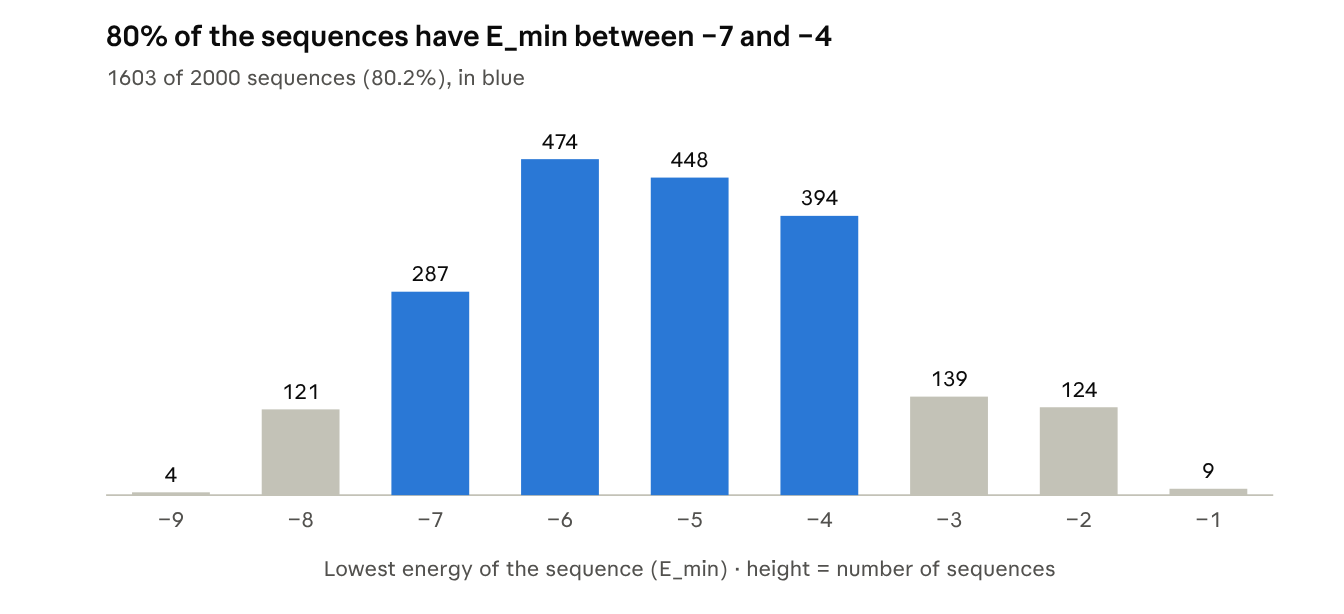
\includegraphics[width=1\textwidth]{images/emin_distribution.png}
  \caption{Distribuzione di $\Emin$ tra le 2000 sequenze.}
  \label{fig:emin}
\end{figure}

Come mostra la figura~\ref{fig:emin}, le energie estreme sono rare: solo 4 sequenze hanno $\Emin = -9$ e 9 hanno $\Emin = -1$. Le metriche calcolate per queste energie si basano quindi su pochi esempi.

\subsection{Confronto tra modello e baseline}
\label{sec:ris-confronto}

Il modello GNN + CNN 1D supera tutte e tre le baseline (tabella~\ref{tab:confronto}). Si ha il 98,1\% di accuratezza sul test, contro il 96,5\% della migliore baseline (B1b) e il 79,3\% della sola energia (B0a).

\begin{table}[htbp]
  \centering
  \caption{Prestazioni sul test set del modello principale e delle baseline.}
  \label{tab:confronto}
  \small
  \begin{tabular}{l>{\raggedright\arraybackslash}p{5.2cm}ccc}
    \toprule
    Modello & Input usato & Accuratezza & AUROC & \begin{tabular}[c]{@{}c@{}}AUROC\\per sequenza\end{tabular} \\
    \midrule
    \textbf{GNN + CNN 1D} & grafo dei contatti + sequenza                    & \textbf{98,1\%} & \textbf{0,999} & 1,000 \\
    B1b (MLP)             & contatti H--H + sequenza, senza struttura a grafo & 96,5\%          & 0,995          & 1,000 \\
    B0b (logistica)       & energia + 5 caratteristiche della sequenza       & 92,0\%          & 0,975          & 1,000 \\
    B0a (logistica)       & sola energia                                     & 79,3\%          & 0,871          & 1,000 \\
    \bottomrule
  \end{tabular}
\end{table}

\paragraph{AUROC per sequenza.} Calcolato separatamente dentro ogni sequenza, vale 1 per tutti i modelli, B0a compresa, e quindi non li distingue (sezione~\ref{sec:impara}).

\paragraph{AUROC.} Su tutte le sequenze insieme sale da 0,871 (B0a) a 0,999 (GNN). La GNN stima $\Emin$ con un errore medio assoluto di 0,27 unità. Sul validation l'AUROC della GNN raggiunge il massimo all'epoca 24, e l'addestramento si ferma all'epoca 34.

\paragraph{Accuratezza.} Le poche caratteristiche della sequenza aggiunte da B0b valgono 12,7 punti rispetto a B0a, e la GNN arriva al 98,1\%. L'accuratezza della GNN passa dal 99,4\% in validation al 98,1\% sul test, che contiene solo sequenze mai viste. Il calo è di appena 1,3 punti, quindi il modello generalizza bene a sequenze nuove.

\subsection{Prestazioni per fascia di difficoltà}
\label{sec:ris-fasce}

Le fasce near e le trappole cinetiche separano i modelli (figura~\ref{fig:fasce}). La GNN le classifica correttamente nel 98\% dei casi, mentre B0a scende al 44\% sui near. I decoy mid e far sono invece facili per tutti infatti anche la sola energia ne riconosce il 91--100\%.

\begin{figure}[htbp]
  \centering
  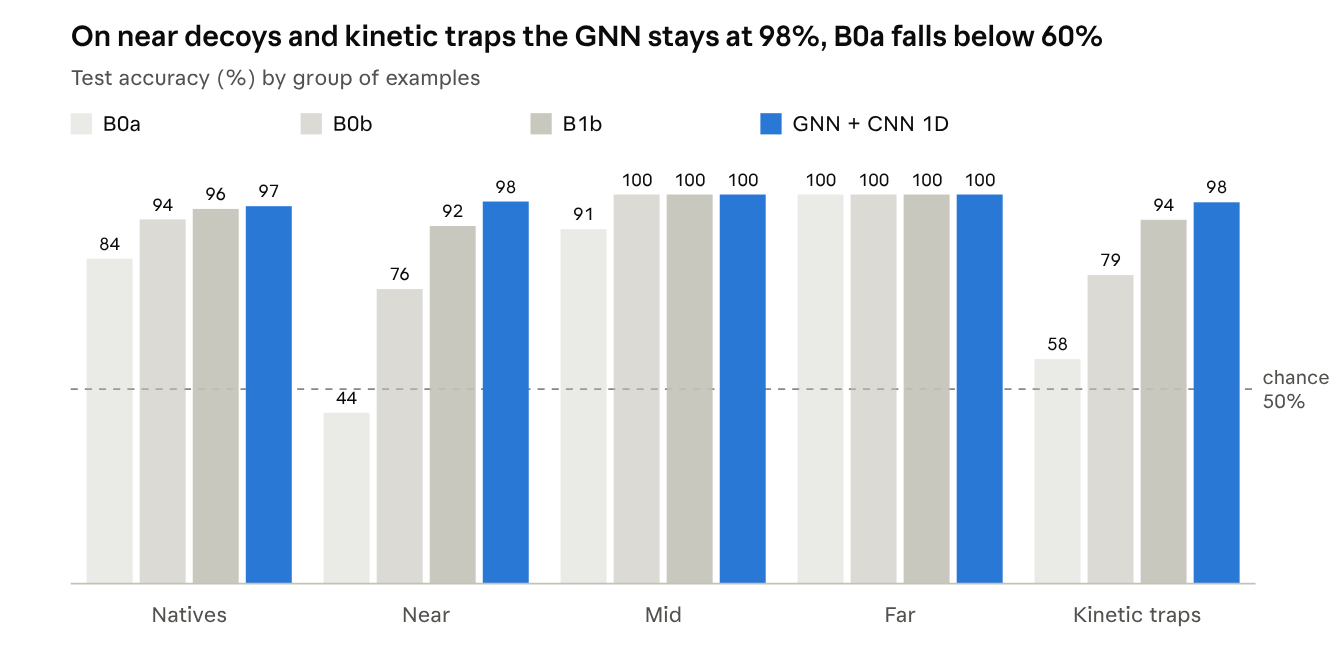
\includegraphics[width=1\textwidth]{images/accuracy_by_tier.png}
  \caption{Accuratezza di test per fascia di difficoltà.}
  \label{fig:fasce}
\end{figure}

Il calo di B0a sui near è atteso. Un decoy near ha energia vicina al minimo della propria sequenza, e senza stimare $\Emin$ un modello non può distinguerlo da un nativo di un'altra sequenza. La GNN mantiene un'accuratezza tra il 96,3\% e il 100\% per ogni valore di $\Emin$, quindi non dipende da quanto è profondo il minimo.

Sui 6230 esempi di test la GNN sbaglia 117 volte: 95 nativi classificati come decoy e 22 decoy near classificati come nativi. Gli errori sono concentrati in 23 delle 200 sequenze di test, e le 5 sequenze peggiori ne raccolgono 74 (63\%). Sui nativi rifiutati la GNN stima in media un $\Emin$ più basso di 0,39 unità rispetto a quello vero. Un esempio è \texttt{PPPPHPPHHHHHHHHH}, con $\Emin = -5$ stimato a $-5{,}42$.

% =====================================================================
\section{Discussione e limiti}
\label{sec:discussione}

I risultati rispondono in modo affermativo alla domanda della sezione~\ref{sec:obiettivi}, entro i limiti discussi nella sezione~\ref{sec:limiti}.

\subsection{Il REMC produce un dataset valido?}
\label{sec:valido}

Sì, per catene di 16 residui. La validità poggia su tre fatti.

\paragraph{Le etichette sono corrette.} Il REMC ha raggiunto il minimo esatto in tutte le sequenze, quindi con 5 repliche e 500 cicli la ricerca è più che sufficiente per $N = 16$. La certezza delle etichette viene però dall'enumerazione esatta, non dal REMC da solo.

\paragraph{I decoy sono difficili.} Più della metà è vicina al minimo e un terzo è una trappola cinetica. Sono gli stati in cui il REMC stesso passa prima di arrivare al minimo, mentre un dataset di conformazioni casuali conterrebbe soprattutto decoy lontani, facili da scartare.

\paragraph{Il modello generalizza.} Le sequenze di test sono del tutto nuove, quindi il modello non può ricordarne i nativi e deve stimare $\Emin$ da solo. Il piccolo calo rispetto al validation mostra che ci riesce.

\subsection{Che cosa impara il modello}
\label{sec:impara}

Il problema si riduce quasi del tutto a stimare $\Emin$ dalla sequenza. Lo mostra l'AUROC per sequenza, che vale 1 per tutti i modelli, compresa B0a infatti dentro una stessa sequenza l'energia basta a ordinare nativi e decoy. La difficoltà nasce solo nel confronto tra sequenze diverse. Per esempio, una conformazione con $E(c) = -4$ è un nativo se $\Emin = -4$, ma un decoy se $\Emin = -7$. Senza stimare $\Emin$ il modello non può decidere.

La scala delle baseline indica quale informazione serve davvero:
\begin{itemize}
  \item \textbf{B0a $\to$ B0b (+12,7 punti).} Pochi conteggi degli H in posizione pari e dispari bastano a stimare in modo grezzo quanto in basso può arrivare l'energia. È il guadagno più grande della scala.
  \item \textbf{B0b $\to$ B1b (+4,5 punti).} Conoscere la sequenza completa e i contatti H--H, non solo i conteggi, rende la stima di $\Emin$ più precisa.
  \item \textbf{B1b $\to$ GNN + CNN 1D (+1,6 punti).} A parità di informazione, l'architettura che segue la catena aggiunge un guadagno piccolo ma netto. Si vede soprattutto sui decoy near e sulle trappole, le fasce che separano i modelli (sezione~\ref{sec:ris-fasce}).
\end{itemize}

Il modello principale si comporta quindi come uno stimatore di $\Emin$ appreso, affiancato dal confronto con l'energia della conformazione. L'errore medio di 0,27 unità su $\Emin$ è coerente con questa lettura.

\subsection{Dove il modello sbaglia}
\label{sec:errori}

Gli errori della GNN sono pochi, sbilanciati e concentrati (sezione~\ref{sec:ris-fasce}). Il fatto che i nativi rifiutati sono molti più dei decoy accettati indica che il modello tende a essere prudente e, nel dubbio, assegna l'etichetta di decoy.

La causa è quella individuata nella sezione~\ref{sec:impara}. Sui nativi rifiutati il modello stima un $\Emin$ più basso di quello vero. Crede cioè che la sequenza possa compattarsi di più, e giudica il vero nativo un decoy.

Gli errori non sono distribuiti a caso. Il caso di \texttt{PPPPHPPHHHHHHHHH}, con nove H consecutivi, suggerisce che si tratti di sequenze poco rappresentate nel train. Con H scelto con probabilità 0,5, blocchi così lunghi sono rari, e il ramo della sequenza ha pochi esempi da cui imparare il loro $\Emin$.

Le trappole cinetiche, che dovevano essere i decoy più difficili, non mettono in crisi la GNN, ma restano decisive per separare i modelli.

\subsection{Limiti}
\label{sec:limiti}

I risultati valgono per le condizioni in cui sono stati ottenuti, e alcune di queste ne limitano la portata.
\begin{itemize}
  \item \textbf{Modello semplificato.} Il reticolo quadrato 2D e l'alfabeto di due lettere sono molto lontani da una proteina reale. Il progetto studia i principi del folding, non prevede strutture vere.
  \item \textbf{Lunghezza fissa e verifica esatta limitata.} Tutte le sequenze hanno 16 residui, e non si sa come il modello si comporti su catene di altra lunghezza. Oltre circa 20 residui l'enumerazione esatta non è più possibile e  le etichette dipenderebbero dal solo REMC, che non garantisce il minimo globale.
  \item \textbf{Sequenze casuali e stati degeneri.} Le sequenze casuali sono spesso molto degeneri (37 stati nativi in mediana), mentre le proteine naturali, selezionate dall'evoluzione, hanno di solito un'unica struttura nativa. Inoltre il REMC non trova necessariamente tutti gli stati degeneri e il tetto di 20 nativi è stato raggiunto dal 64,7\% delle sequenze, quindi il dataset copre solo una parte degli stati nativi possibili.
  \item \textbf{Decoy dello stesso generatore.} Nativi e decoy provengono dallo stesso REMC. Il modello potrebbe comportarsi peggio su decoy prodotti in altro modo, per esempio da un altro algoritmo di ricerca.
  \item \textbf{Vantaggio pratico ridotto a $N = 16$.} Per catene così corte l'enumerazione esatta è già abbastanza rapida, quindi un modello che evita il REMC serve più come prova di principio che come strumento. Il vantaggio diventerebbe concreto solo su catene più lunghe, dove però valgono i limiti precedenti.
\end{itemize}

% =====================================================================
\section{Conclusioni e sviluppi futuri}
\label{sec:conclusioni}

\subsection{Conclusioni}

Il progetto si chiedeva se il REMC fosse in grado di produrre un dataset valido per addestrare un classificatore di conformazioni native (sezione~\ref{sec:obiettivi}). Per catene HP di 16 residui sul reticolo quadrato 2D la risposta è \textbf{sì} essendo che il REMC ha raggiunto il minimo esatto in tutte le sequenze e ha prodotto decoy in gran parte vicini al minimo, proprio i casi che rendono il compito non banale.

Il modello GNN + CNN 1D addestrato su questo dataset classifica correttamente il \textbf{98,1\%} delle conformazioni di sequenze mai viste (AUROC 0,999) e supera tutte le baseline. Il confronto con le baseline mostra che il compito si riduce quasi del tutto a \textbf{stimare $\boldsymbol{\Emin}$ dalla sequenza}.

\subsection{Sviluppi futuri}

Gli sviluppi più utili rispondono ai limiti della sezione~\ref{sec:limiti} e agli errori della sezione~\ref{sec:errori}.
\begin{itemize}
  \item \textbf{Catene più lunghe e di lunghezza variabile.} La GNN lavora su grafi di qualsiasi dimensione, quindi può essere addestrata su sequenze di lunghezze diverse. Oltre i 20 residui le etichette andrebbero controllate in altro modo, per esempio con più esecuzioni indipendenti del REMC. È qui che il modello darebbe un vantaggio pratico rispetto alla ricerca diretta.
  \item \textbf{Reticoli diversi.} Lo stesso schema si può applicare al reticolo cubico 3D, adattando le mosse del REMC e la costruzione della mappa dei contatti.
  \item \textbf{Sequenze poco rappresentate.} Si potrebbero generare più sequenze con lunghi blocchi di H, o variare la probabilità di H, così che il ramo della sequenza veda più esempi da cui stimare $\Emin$.
  \item \textbf{Decoy da altri generatori.} Per verificare che il modello non dipenda dal REMC, lo si può valutare su decoy prodotti in altro modo, per esempio da un Monte Carlo a temperatura singola.
  \item \textbf{Il modello come supporto alla ricerca.} La stima di $\Emin$ data dal ramo della sequenza potrebbe servire al REMC stesso, per esempio per fermare la simulazione quando una conformazione raggiunge l'energia prevista.
\end{itemize}

% =====================================================================
\newpage
\begin{thebibliography}{9}

%\bibitem{anfinsen1973}
%C.~B. Anfinsen.
%\newblock Principles that govern the folding of protein chains.
%\newblock \emph{Science}, 181(4096):223--230, 1973.

%\bibitem{dill1985}
%K.~A. Dill.
%\newblock Theory for the folding and stability of globular proteins.
%\newblock \emph{Biochemistry}, 24(6):1501--1509, 1985.

%\bibitem{lesh2003}
%N.~Lesh, M.~Mitzenmacher e S.~Whitesides.
%\newblock A complete and effective move set for simplified protein folding.
%\newblock In \emph{Proceedings of the 7th Annual International Conference on Research in Computational Molecular %Biology (RECOMB)}, pp.~188--195, 2003.

%\bibitem{thachuk2007}
%C.~Thachuk, A.~Shmygelska e H.~H. Hoos.
%\newblock A replica exchange {M}onte {C}arlo algorithm for protein folding in the {HP} model.
%\newblock \emph{BMC Bioinformatics}, 8:342, 2007.

\end{thebibliography}

\end{document}
